%! Author = melek
%! Date = 29.12.2022

% Preamble
\documentclass[11pt]{article}

% Packages
\usepackage{amsmath}
\usepackage{graphicx}
\graphicspath{ {../images/} }

\title{Assignment 1: Imitation Learning}
\author{huseyinabanox@gmail.com}
\date{June 2022}

% Document
\begin{document}

    \maketitle

    \section{Behavioral Cloning}

    \subsection{Answer}

    Following files are modified:

    - rl\_trainer.py

    - bc\_agent.py

    - MLP\_policy.py

    - replay\_buffer.py

    - utils.py

    - pytorch\_utils.py

    \subsection{Answer}


    \noindent eval\_batch\_size                                 5000

    \noindent ep\_len                                           1000

    \noindent num\_agent\_train\_steps\_per\_iter               1000

    \noindent n\_layers                                         2

    \noindent size                                              64

    \noindent learning\_rate                                    0.0005


    \begin{table}[]
        \begin{tabular}{lllll}
                                 & Hopper & Ant   & HalfCheetah & Walker2d \\
            Eval\_AverageReturn  & 961    & 4604  & 4009        & 441      \\
            Eval\_StdReturn      & 285    & 91    & 67          & 325      \\
            Train\_AverageReturn & 3773   & 4714  & 4206        & 5567     \\
            Train\_StdReturn     & 2      & 12    & 83          & 9        \\
            Log\_Loss            & -351   & -1518 & -804        & -507
        \end{tabular}
    \end{table}

    \subsection{Answer}

    Walker2d is performing worst.
    Mean and std results indicate learning is not happening.
    First thing to play with is the learning rate.
    After finding a reasonable LR, then training steps are adjusted.

    \hspace*{-1.5in}
    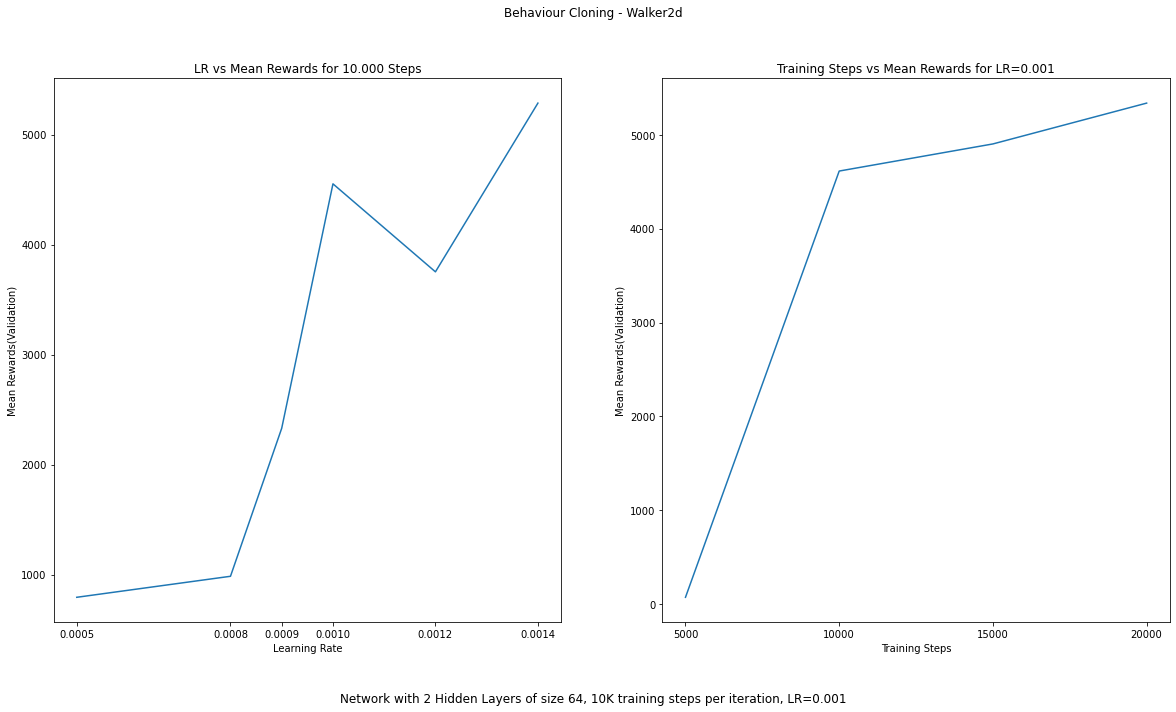
\includegraphics[scale=0.4]{q1.3_plots}

\end{document}